\documentclass{ximera}  


\input{../preamble.tex}



 
\title{Inductance} 
\author{Milica Markovic} 
\outcome{Inductors.}
\begin{document}  
\begin{abstract}  

\end{abstract}  
\maketitle    

\subsection{Mutual Inductance}


\begin{figure}[htbp]
\begin{center}
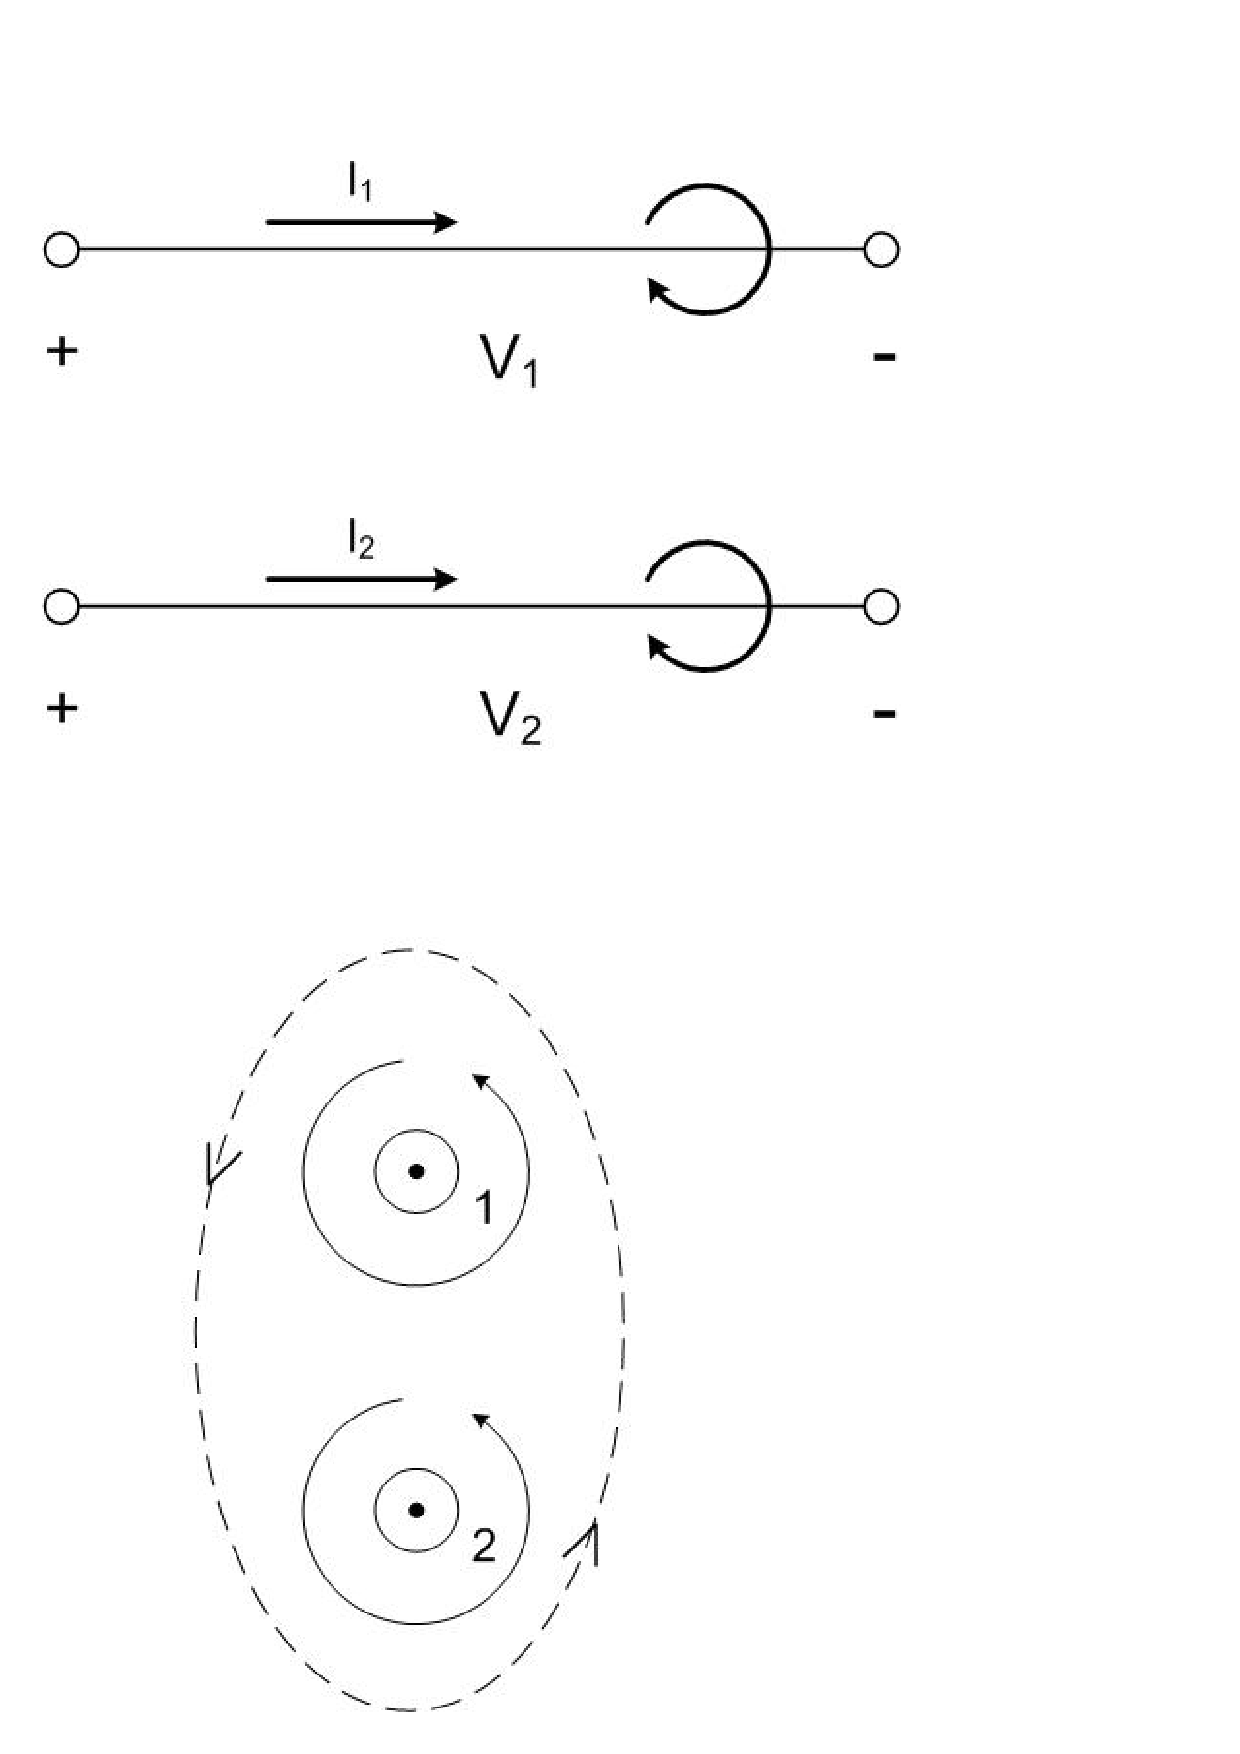
\includegraphics[scale=0.5]{../jpg/increaseinflux.jpg}
\end{center}
\caption{Mutual Inductance: Increasing the magnetic field and therefore current in one wire due to another wire in vicinity. }
\label{MutualInduc}
\end{figure}



\subsection{Inductance in circuit theory}


\begin{figure}[htbp]
\begin{center}
\includegraphics[scale=0.5]{../jpg/CircuitwithInductor.jpg}
\end{center}
\caption{Simple electronic circuit with an inductance and resistance. }
\label{MutualInduc}
\end{figure}










\end{document} 
